\documentclass[11pt,letterpaper]{article}
\usepackage[english]{babel}
\usepackage[utf8]{inputenc}
\usepackage{fancyhdr}
\usepackage[margin=1in]{geometry}
\usepackage{enumitem}
\usepackage{amsmath}
\usepackage{graphicx}
\usepackage{setspace} 
\onehalfspacing
 
\pagestyle{fancy}
\fancyhf{}
\lhead{STAT 423 HW 3}
\rhead{Nan Tang (1662478)}
\rfoot{Page \thepage}
 

\title{STAT 423 Homework 3}
\author{Nan Tang 1662478}
\date{\today}

\begin{document}

\maketitle
\section*{1}
\subsection*{a}

\noindent At the significance level of $5 \%$, base on p-value of t-test, predictors RV, CA, FIA, CTA have significant effects on returns of FoHF. Among these significant factors, RV has negative impact, while others have positive impact, since estimated coefficient for RV is negative and are positive for others. \\

\noindent the small p-value of F test rejects the null hypothesis that all the predictors have no effect on FoHF, implying there is at least on significant factors among all these predictors that have impact. \\

\noindent R square represents goodness of fitting a linear regression on the data. The relatively large R-square in this case, $0.7798$, implies linear regression may be a good fit for the FoHF data. 

\subsection*{b}
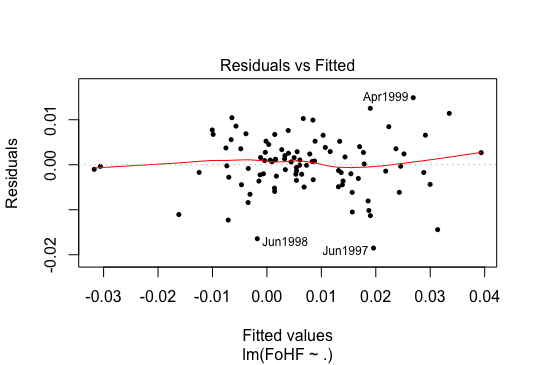
\includegraphics[scale=0.7]{1-b-1.png}

\noindent The TA plot shows an approximately horizontal line on zero, indicating the assumption of zero expected value for error is not violated. The width of residuals around zero line slightly increases as fitted value increases. This pattern implies the constant variance assumption might be violated. The distribution of residuals does not show particular pattern, therefore, assumption of independence is not violated.\\

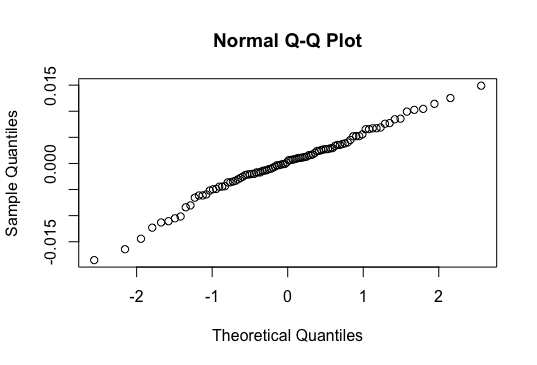
\includegraphics[scale=0.7]{1-b-2.png}

\noindent QQplot shows approximately linear pattern, indicating the residuals follow normal distribution. Therefore the normality assumption of error is not violated. \\

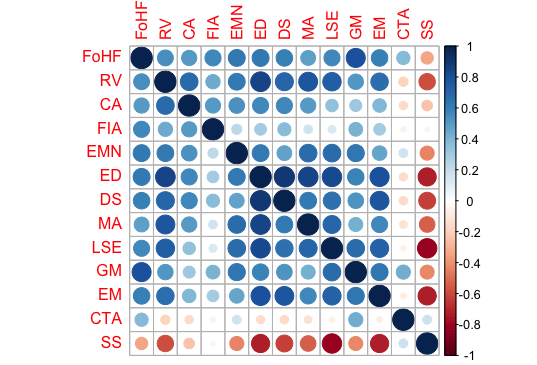
\includegraphics[scale=0.7]{1-b-3.png}

\begin{verbatim}
> vif(fit1)
       RV        CA       FIA       EMN        ED        DS 
 6.387024  2.982646  2.271113  3.672017 29.973694  9.404810 
       MA       LSE        GM        EM       CTA        SS 
 8.001994 10.046374  5.699120  4.255477  2.232320  4.972861 
\end{verbatim}

\noindent From the correlation matrix, we can perceive that predictor RV have strong correlation with other predictors such as ED, MA, LSE, EM and SS; ED is strongly correlated with DS, MA, LSE, EM, SS; DS is strongly correlated with EM. \\

\noindent The serious issue with multicollinearity can also be reflected on VIF values of predictors. ED, LSE, DS all have VIF values more than 5. 

\subsection*{c}
\noindent To solve the unequal variance problem, I will transform data of response variable via box-cox transformation. Multi-collinearity is the most serious problem. To fix this issue, I will keep ED and delete all other predictors that are strongly correlated with ED, such as RA, DS, MA, LSE, EM, SS. 

\subsection*{d}
\textbf{Backward Selection}
\begin{verbatim}
fit1 <- lm(formula=FoHF ~., data=FoHF)
step(object=fit1, direction='backward', k=log(nrow(FoHF)))

## result 
Call:
lm(formula = FoHF ~ CA + FIA + ED + GM + CTA, data = FoHF)

Coefficients:
(Intercept)           CA          FIA           ED           GM          CTA  
  -0.001857     0.175665     0.298492     0.265442     0.246942     0.153503  
\end{verbatim}

\noindent If start from full model and use BIC criterion, the correct model will contain predictors CA, FIA, ED, GM, CTA. \\

\noindent \textbf{Forward Selection}
\begin{verbatim}
fit2 <- lm(formula=FoHF ~ , data=FoHF)
step(object=fit2, direction='forward', k=log(nrow(FoHF)), scope=list(upper=fit1, lowwer=fit2))


## result
Call:
lm(formula = FoHF ~ GM + CA + FIA + CTA + ED, data = FoHF)

Coefficients:
(Intercept)           GM           CA          FIA          CTA           ED  
  -0.001857     0.246942     0.175665     0.298492     0.153503     0.265442  

\end{verbatim}

\noindent If start from empty model and use BIC criterion, the correct model will contain GM, CA, FIA, CTA, ED. 

\noindent \textbf{All Subset Selection}
\begin{verbatim}
regsub_out <- regsubsets(FoHF~., data=FoHF)
summary(regsub_out)$bic

Selection Algorithm: exhaustive
         RV  CA  FIA EMN ED  DS  MA  LSE GM  EM  CTA SS 
1  ( 1 ) " " " " " " " " " " " " " " " " "*" " " " " " "
2  ( 1 ) " " "*" " " " " " " " " " " " " "*" " " " " " "
3  ( 1 ) " " " " "*" " " "*" " " " " " " " " " " "*" " "
4  ( 1 ) " " " " "*" " " "*" " " " " " " "*" " " "*" " "
5  ( 1 ) " " "*" "*" " " "*" " " " " " " "*" " " "*" " "
6  ( 1 ) "*" "*" "*" " " "*" " " " " " " "*" " " "*" " "
7  ( 1 ) "*" "*" "*" " " "*" " " " " "*" "*" " " "*" " "
8  ( 1 ) "*" "*" "*" " " "*" " " " " "*" "*" " " "*" "*"

> which(summary(regsub_out)$bic == min(summary(regsub_out)$bic))
[1] 5
\end{verbatim}

\noindent The model that has minimum BIC is model 5, which contains CA, FIA, ED, GM, CTA. \\

\noindent \textbf{conclusion:} The procedure of forward, backward and all subset shows the best model based on BIC value is the model that contains  predictors CA, FIA, ED, GM, CTA. 

\section*{2}
\subsection*{a}

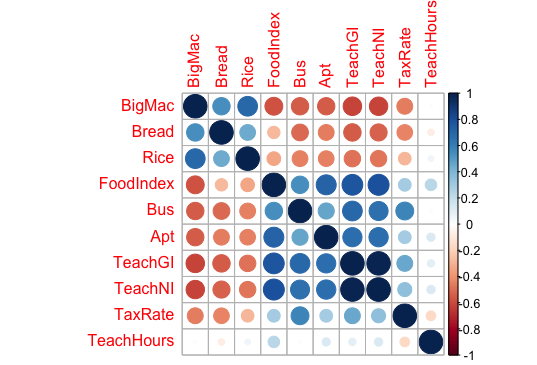
\includegraphics[scale=0.8]{2-a-1.png}

\noindent Base on the correlation matrix, predictor TeachNI has strong co-linearity with TeachGI (approximately 1). Strong multi-colinearity may exist between FoodIndex, Bus, Apt, TeachNI and TeachGI.

\subsection*{b}
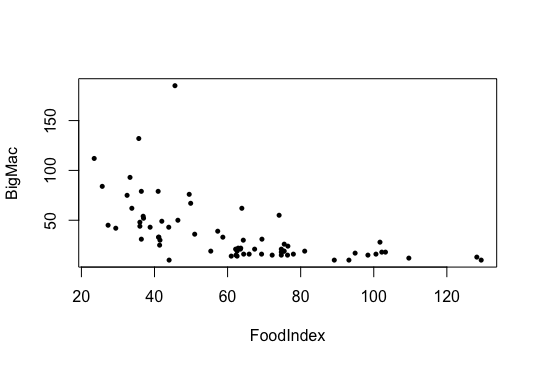
\includegraphics[scale=0.7]{2-b-1.png}

\noindent Without any data transformation, the scatterplot shows non-linear (more like exponential distribution) relationship between FoodIndex and BigMac. 

\subsection*{c}
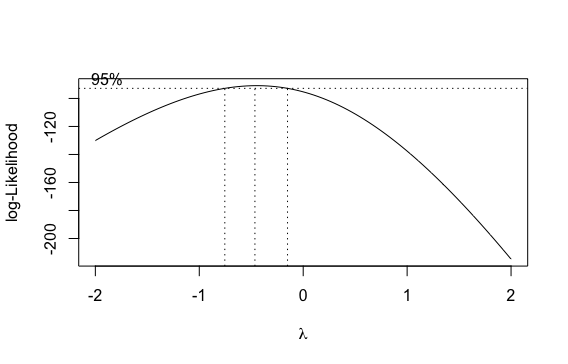
\includegraphics[scale=0.7]{2-c-1.png}

\noindent $\lambda$ for maximum log-likelihood is equal to -0.4646, however, considering -0.5 also falls in $95 \%$ confidence interval, we can transform response variable $y \rightarrow \frac{1 - log^{-1}(y) }{0.5}$

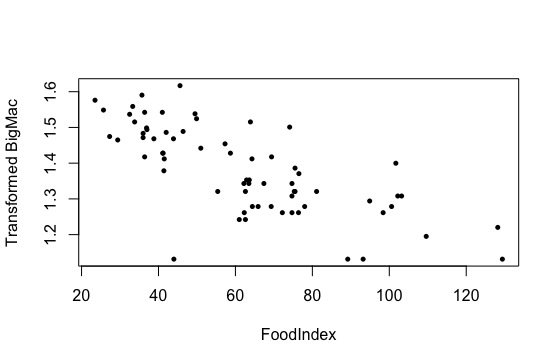
\includegraphics[scale=0.7]{2-c-2.png}

\noindent The scatter plot looks better as linear relation exists after transformation. 

\subsection*{d}
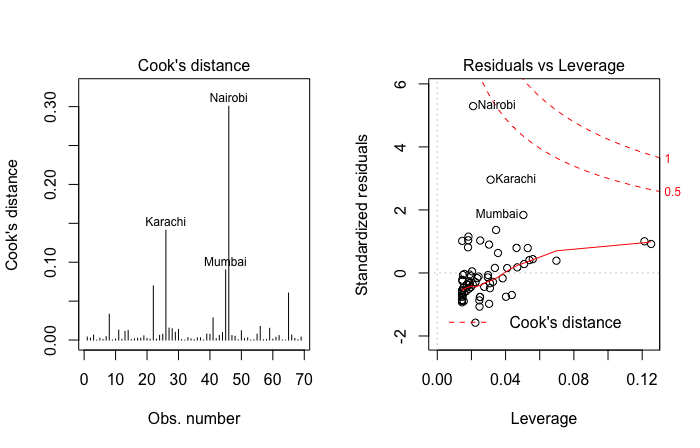
\includegraphics[scale=0.6]{2-d-1.png}

\noindent Base on Cook's distance, cities named as Nairobi ($\approx 0.3$) and Karachi ($\approx 0.15$) have largest influence on fitted line. 

\subsection*{e}
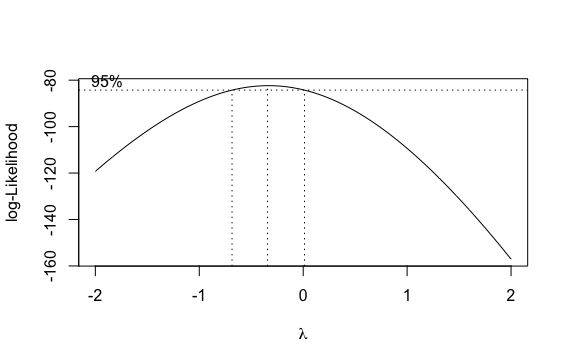
\includegraphics[scale=0.7]{2-e-1.png}

\noindent In the reduced dataset, $\lambda$ for maximum log-likelihood changes to $-0.3434$. Since the $95 \%$ confidence for $\lambda$ covers zero, we can transform response variable $y \rightarrow log(y)$.

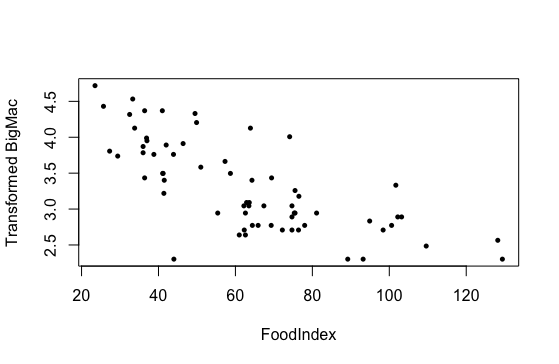
\includegraphics[scale=0.7]{2-e-2.png}

\subsection*{f}
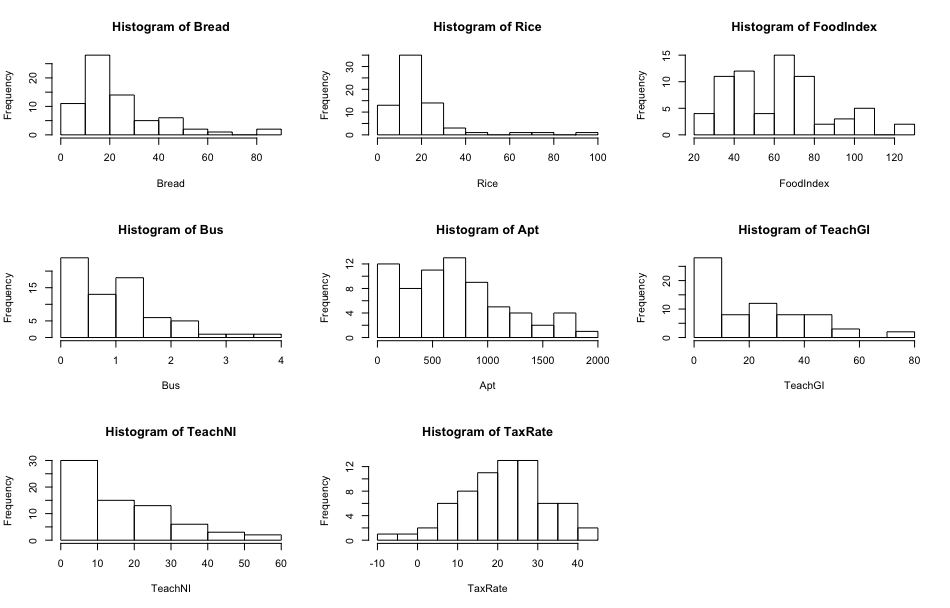
\includegraphics[scale=0.5]{2-f-1.png}

\noindent Distributions of Bread, Rice, Bus, Apt, TeachGI, TeachNI are right skewed.

\subsection*{g}
\begin{verbatim}
> c(loocv.lm(model1), loocv.lm(model2), loocv.lm(model3))
[1] 0.1984310 0.1353951 0.1008867
\end{verbatim}

\noindent Base on LOOCV values of three models, model 3 which contains all predictors log(Bread), log(Rice), Apt, log(Bus), log(TeachNI) has the best score. 

\subsection*{h}
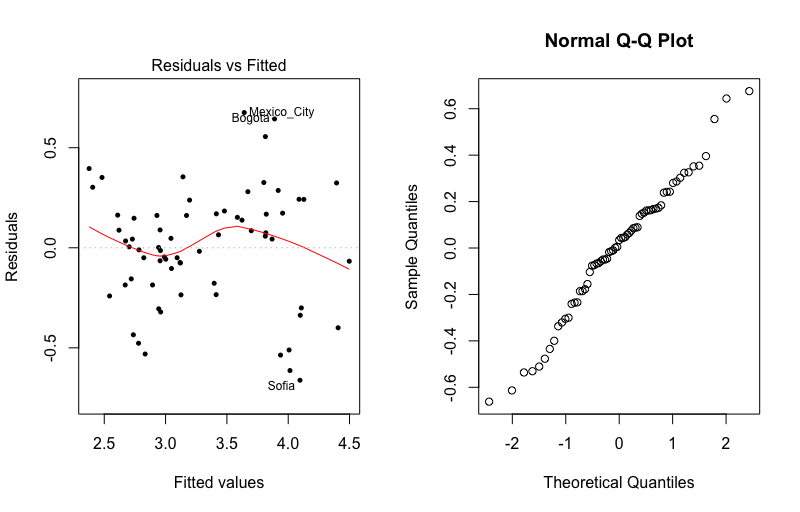
\includegraphics[scale=0.5]{2-h-1.png}

\noindent Normality, independence and zero mean assumptions of error are not violated, However, the variance of residuals is not constant along with fitted value. The assumption for constant error variance might be violated. 

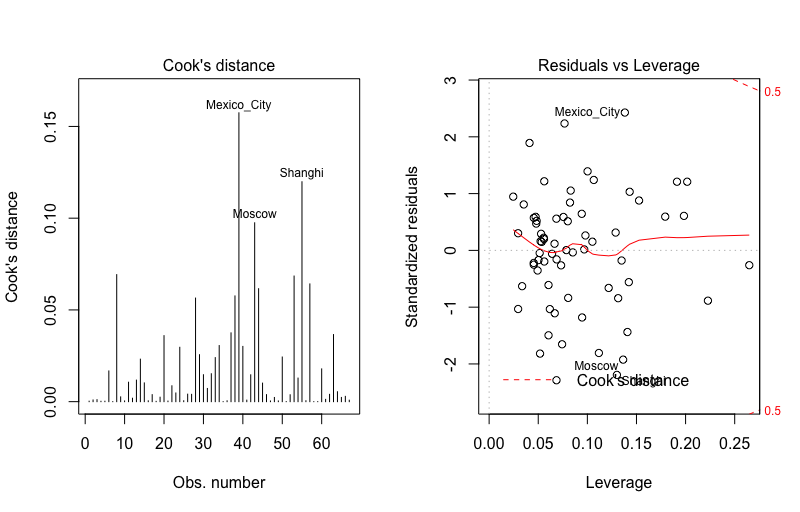
\includegraphics[scale=0.5]{2-h-2.png}

\noindent Cook's distance for all data points are below 0.15 after transformation of response variable. There is no effect from outliers. 

\section*{3}

\begin{enumerate}[label=(\alph*)]
\item choose a) \\
since interaction of $X_2$ and $ X_3$, $ X_4$ and $ X_5$ are significant, by hierarchy principle, theses main factors should be included in model. 

\item choose d) \\
if model exclude $X_2, X_3, X_6$, AIC will inflate, therefore these three factors should be included. Adding any other predictors will slightly inflate AIC, therefore, none of the others should be added. 

\item choose d) \\
information of sample size is missing, therefore cannot compare BIC scores with AIC scores.

\item choose c) \\
M1 which contains none of the predictors has worst AIC score. 

\item choose d) \\
adding predictors will increase goodness of fit. 

\end{enumerate}

\section*{4}

\begin{enumerate}[label=(\alph*)]
\item choose a) \\
result of global F-test cannot be used to conclude all predictors are significant. 

\item choose b) \\
p-value and confidence interval are complementary. 

\item choose b) 

\item choose c) \\
qqplot can check normality assumption of error. 

\item choose b) \\
larger sample size leads to smaller standard error and larger test statistics, thereby having a smaller p-value. 


\end{enumerate}



\end{document}